\documentclass[10pt,twocolumn,letterpaper]{article}

\usepackage{cvpr}
\usepackage{times}
\usepackage{epsfig}
\usepackage{graphicx}
\usepackage{amsmath}
\usepackage{amssymb}

% Include other packages here, before hyperref.

% If you comment hyperref and then uncomment it, you should delete
% egpaper.aux before re-running latex.  (Or just hit 'q' on the first latex
% run, let it finish, and you should be clear).
\usepackage[pagebackref=true,breaklinks=true,letterpaper=true,colorlinks,bookmarks=false]{hyperref}

\cvprfinalcopy % *** Uncomment this line for the final submission

\def\cvprPaperID{****} % *** Enter the CVPR Paper ID here
\def\httilde{\mbox{\tt\raisebox{-.5ex}{\symbol{126}}}}

% Pages are numbered in submission mode, and unnumbered in camera-ready
\ifcvprfinal\pagestyle{empty}\fi
\begin{document}

%%%%%%%%% TITLE
\title{Institute Vaccine Management Solution }

\author{Ashish Gupta\\
International Institute of Information and Technology Hyderabad\\
% Institution1 address\\
{\tt\small ashish.gupta@students.iiit.ac.in}
% For a paper whose authors are all at the same institution,
% omit the following lines up until the closing ``}''.
% Additional authors and addresses can be added with ``\and'',
% just like the second author.
% To save space, use either the email address or home page, not both
% \and
% Second Author\\
% Institution2\\
% First line of institution2 address\\
% {\tt\small secondauthor@i2.org}
}

\maketitle
%\thispagestyle{empty}

%%%%%%%%% ABSTRACT
\begin{abstract}
   The onset of the second wave of the double  mutant Covid-19 coronavirus has led to a increase in necessity of vaccination of all people.The only way for life to come back to normal is through efficient vaccination of young and elderly.This paper proposes a software system providing solutions to design a platform that can manage mass vaccination,including distribution and prioritization.
\end{abstract}

%%%%%%%%% BODY TEXT
\section{Introduction}

India recorded more than 400,000 new COVID-19 cases for the first time on May First~\cite{Cases1} as it battles a devastating second wave.With the exponential increase in number of cases in the country,everyone is finding it difficult to manage the large inflow of patients.The surge has overwhelmed hospitals, morgues and crematoriums,left families scrambling for scarce medicines and oxygen and increased the importance of vaccination of one and all.
\begin{figure}[h]
    \centering
    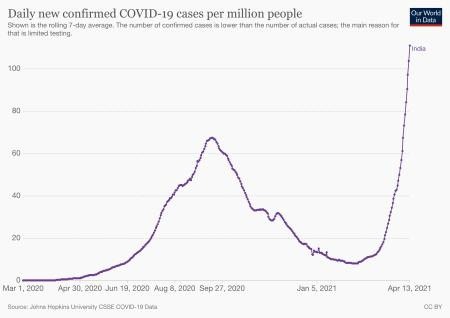
\includegraphics[width=2.6in, height=2.6in]{1.jpeg}
    \caption{Confirmed Cases per million people ~\cite{Photo}}
\end{figure}
The sheer massivenes of the Vaccination drive brings problems with itself.Vaccine data capture cannot be be on paper and will have to be digitalized In vaccine delivery, the challenge is ensuring there is a demand for services in those who are most at risk. There is also the challenge of prioritization. There are issues related to financial and human resources required and expansion related to cold chain infrastructure.Existing systems need to be fast enough to cater to the high capacity booking.Also with a large receipants, each dose will need to be tracked and verified to ensure that counterfeits don't come into play.

With the recent increase in covid cases on campus and around 400 people on campus, and with the already occupied Aarogya doctors and nurses,
manually managing doses within a short period can be a mess.There is a need for procurement for all age, a centralized solution for mass -management of Vaccination.
%-------------------------------------------------------------------------
\section{Literature Review}
\subsection{Introduction}
Several organizations have created services for optimized management of vaccination solutions.Most of these services include vaccination slot management or tracking and analysing the vaccine administering and requirements.

\subsection{Accenture Solutions }

The Accenture Vaccine Management Solution consists of five basic modules and consulting support that can be used together or individually.It starts with Supply Management taking benefit from the Accenture's extensive supply chain experience and goes all the way to Vaccine Management and Tracking Platform leverages Salesforce’s manual contact tracing solution.It brings together Accenture’s industry, analytics and consulting experience and includes components built on the Salesforce platform.~\cite{Accenture}

\subsection{Deloitte}
The Vaccine Management solution prepared by Deloitte works on a centralized vaccination platform.It is designed to provide real-time access to vaccine administration data to support decision-making, including support for outreach campaigns.The Vaccine recipients can look up and schedule appointments,access their immunization certificate and report any adverse events which is the forwarded to higher authorities.~\cite{Delloitte}
\subsection{Infosys Public Services}
IPS combined with Simplus and Salesforce have developed a solution to offer modular platform for governments.The IPS platform forecasts the vaccine demand and prioritizes through consolidation of testing, tracing, and vaccine data.It includes epidemiological insights for improved policy and decision making.The resident community is the one-stop-shop for individuals to find information, register with state and local governments, and schedule vaccine appointments. The provider community is the central hub for providers. ~\cite{Infosys}
%%%%%%%%%%%%%%%%%%%%%%%%%%%%%%%%%%%%%%%%%%%%%%%%%%%%%%%%%%%%%%%%%%%%%%%%%%%%%%%%%%%%
\section{System Architecture}
\subsection{Overview}
The content of the software is described and demonstrated by the software architecture.
The proposed solution hosted on college server can be accessed from various platforms such as Websites,Mobile applications etc.The application has following key components
\begin{itemize}
    \item Frontend : A simple UI that can be used by people of all ages to display availability and booking of slots,to perform pre-screening tests and viewing/downloading a digital signature as a proof of immunization.
    \item Notifier:To remind users of their scheduled appointment and the Healthcare workers in the case of absence of vaccines
    \item Backend : It handles the user requests and communicates with prioritization model and prediction model and perform the necesary calls.
    \item Prioritization model : Prioritizes users based on the risk associated with them on various parameters.
    \item Prediction model: Predicts the need to order vaccines on various input parameters.
    \item Database : Each user registered is divided into 3 categories namely the vaccine recipients,healthcare workers and CHMC admins.The data of both vaccine recipients and workers can be seen by the admins
\end{itemize}
\subsection{Use Cases}
\subsubsection{User Authorization}
The users upon selecting their role are redirected based upon them.All the vaccine recipients are redirected to login through CAS.Since their Basic Personal information is stored in Institute data,this cuts out the need for Setting up their profile.Similarly Admins can login to view the statistics

The Healthcare staff can login separately as guest.
These users are then redirected to respective Dashboards.
\subsubsection{Dashboard for Vaccine Recipients}
The Dashboard for Vaccine Recipients would consist of the following:
\begin{itemize}
    \item Users will be able to view real-time status of all the available slots and amount of people that registered them
    \item Users can schedule appointments /book up the slots for immunization.These the will receive  a QR code which will be required on vaccination site.
    \item Users can notify authorities in case of any allergies beforehand or adverse events after vaccination.
    \item User will be notified regarding the appointment or in case of any change/postponement of the allotted slot.
    \item Users will be able to download certificates upon complete immunization
\end{itemize}
\subsubsection{Dashboard for HealthCare Workers}
The Dashboard Consists of the following options:
\begin{itemize}
\item Users will be able to see the bookings made in their respective slots
\item The Healthcare Staff will be notified incase of any complications already present in the vaccine recipients.
\item Users can notify the recipients if there is any change in their schedule.
\item The Health Care workers will scan the recipient's code to confirm their immunization
\end{itemize}
\subsubsection{Dashboard for CHMC admins}
\begin{itemize}
\item CHMC admins can view the real-time vaccination status and statistics of all the campus residents.
\item The admins can then restock vaccines and get the probability of them finishing in meantime.
\item They can reschedule slots in case of any events on Campus.
\end{itemize}
\subsection{Models}
\subsubsection{Prioritization Model}
This model prioritizes the vaccine recipients based on epidemiological factors,i.e.their age,past infections,current complications and level of their contact with other people.The model ranks people upon these basis and sends call to backend to update their slots.
\subsubsection{Prediction Model}
This model takes input the consumption of the vaccines and their delivery delays to pre-order the vaccine.Also it takes the current inflow of people in the campus to increase vaccines ordered.
\section{Conclusion}
The solution proposed is efficient and reduces the hassle of screening the vaccine recipients and filling out their personal info.Hope this solution will help authorities in their task of vaccinating one and all.
\subsection{Future Work}
For Future work,we can expand by the usage of blockchain technology to cater for a large amount of people.In addition to this,vaccine providers can be connected for better realization of vaccine data.

{\small
\bibliographystyle{ieee}
\bibliography{egbib}
}

\end{document}
